\documentclass[../UNABRIDGEDalgebraNotesMSRI-UP2016.tex]{subfiles}

\begin{document}

\section[\S \thesection]{Basic definitions}\label{sec:2p1basicDefinitions}
% % % % %
\subsection[\subsecname]{Sets and functions}\label{subsec:setsAndFunctions}
% % %
\begin{frame}{\subsecname}{}
\begin{dfn}\label{dfn:set}
\begin{enumerate}
\item\label{dfnpt:set} 
A \vocab{set} is a well-defined collection of objects called \vocab{elements}.  We write $s\in S$ to mean the element $s$ is in the set $S$.
\item Given any collection of sets $S_1,\dots,S_n$ we can form a \vocab{direct product} 
\[
S_1\times\cdots\times S_n=\{(s_1,\dots,s_n)\mid s_i\in S_i\text{ for each} i=1,\dots,n\},
\]
also a set.  The elements $(s_1,\dots,s_n)$ are called \vocab{$n$-tuples}.
\end{enumerate}
\end{dfn}

\smallGap
In part \lilRefPd{dfnpt:set} of Definition \ref{dfn:set}, \emph{well-defined} is meant in the sense that one cannot give the same name to two different elements.  There is a more typical use of the term which we will make explicit shortly.
\end{frame}

% % % 
\begin{frame}{}{}
\begin{ex}\label{ex:sets}
The following are examples of sets.
\begin{enumerate}
\item $\N=\{1,2,3,\dots\}=$ the \vocab{natural numbers}.  Also denoted $\Z^+$ or $\Z_{>0}$.
\item $\Z=\{0,\pm 1, \pm 2,\dots\}=$ the \vocab{integers}.
\item $\Q=\{\frac{m}{n}\mid m,n\in \Z\text{ and }n\neq 0\}=$ the \vocab{rational numbers}.
\item $\R=$ the \vocab{real numbers}.
\item $\C=$ the \vocab{complex numbers}.
\item $\Mat_{R}(n,n)=$ the set of $n\times n$ matrices with entries in $R=\Z$, $\Q$, $\R$, $\C$, etc.
\item $R^{\times}:=R\setminus\{0\}=$ the \vocab{multiplicative group of $R$}, where $R=\Q$, $\R$, $\C$.
\end{enumerate}
\end{ex}
\end{frame}

% % %
\begin{frame}
\begin{dfn}
\begin{enumerate}
\item A \vocab{function} (or \vocab{map}) $\varphi$ is a rule
\[
\varphi:S\to T
\] 
which assigns each element $s$ in the set $S$ to an element $\varphi(s)$, called its \vocab{image}, in the set $T$.  
\item Given a function $\varphi:S\to T$, $S$ is called the \vocab{domain} (or \vocab{source}) of $\varphi$ and $T$ is called the \vocab{codomain} (or \vocab{target}) of $\varphi$.  
\item The \vocab{image} of a function $\varphi:S\to T$ is the set of elements $t\in T$ such that there exists $s\in S$ satisfying $\varphi(s)=t$.  We use the notation $\varphi(S)$ or $\image(\varphi)$.
\item The set of functions from one set $S$ to another $T$ is called a \vocab{function space}, denoted $T^S$.
\end{enumerate}
\end{dfn}
\end{frame}

% % % 
\begin{frame}[c]{}{}
In order to be \vocab{well-defined} as a function, $\varphi:S\to T$ cannot map the same element $s\in S$ to more than one distinct element in $T$.  

\smallGap
However, we may have $\varphi(s_1)=\varphi(s_2)$ with $s_1\neq s_2$.  

\smallGap
We also do not require every element $t\in T$ to have a \vocab{preimage} in $S$, meaning, there need not exist any $s\in S$ such that $t=\varphi(s)$.

\smallGap
\begin{ex}
Define $\varphi: \Q\to \Z$ by $\varphi(\frac{m}{n})=n$.  Why isn't $\varphi$ well-defined?
\end{ex}
\end{frame}

% % %
\begin{frame}
As one might expect, we have terms to describe such situations where no two elements in $S$ have the same image and/or every element in $T$ has a preimage.

\smallGap
\begin{dfn}\label{dfn:injSurj}
Suppose $\varphi:S\to T$ is a map between sets.
\begin{enumerate}[(a)]
\item\label{dfn:inj} $\varphi$ is \vocab{one-to-one} (or \vocab{injective}) means for all $s_1,s_2\in S$, if $\varphi(s_1)=\varphi(s_2)$ then $s_1=s_2$.
\item\label{dfn:surj} $\varphi$ is \vocab{onto} (or \vocab{surjective}) means for all $t\in T$, there exists $s\in S$ such that $t=\varphi(s)$.
\item $\varphi$ is \vocab{bijective} means it is both injective and surjective.
\end{enumerate}
\end{dfn}

\smallGap
The phrasing of Definition \ref{dfn:injSurj} suggests an approach to proving injectivity and surjectivity.
\end{frame}

% % %
\begin{frame}%[c]{}{}
\begin{ex}\label{ex:expSurj}
The exponential function $f(x)=e^x$, or,  
\begin{align*}
f:\R &\to \R \\
 x &\mapsto e^x,
\end{align*}
is injective.  To prove, suppose $f(x)=f(y)$ for $x,y\in \R$.  Then 
\begin{align*}
e^x &= e^y\; \text{ implies } \\
\ln{(e^x)} &= \ln{(e^y)}\; \text{ implies } \\
x &= y. 
\end{align*}
Thus $x$ and $y$ had to be the same element.
\end{ex}
\end{frame}

% % %
\begin{frame}[c]
On the other hand, the map $f$ in Example \ref{ex:expSurj} is not surjective.

\smallGap
\begin{que}
How would you prove $f$ in Example \ref{ex:expSurj} is not surjective?  How would you change the codomain to make $f$ surjective?
\end{que}
\end{frame}

% % %
\begin{frame}%[c]
\begin{ex}\label{ex:projFunction}
The \vocab{projection map} 
\begin{align*}
\pi: \Z\times \Z &\to \Z \\
 (a,b) &\mapsto a
\end{align*} 
is surjective; to see why, choose any element $x\in\Z$.  Then $x$ has a preimage since, for example, $\pi(x,x)=x$.    
\end{ex}

\smallGap
\begin{que}
Is the projection map $\pi$ in Example \ref{ex:projFunction} injective?  Answer with proof.
\end{que}
\end{frame}

% % %
\begin{frame}[c]
\begin{exe}[cf. Problem 38]\label{exe:functions}
Which of the following are functions?  Of those, which are injective and which are surjective?
\begin{enumerate}[(a)]
\item $\varphi_1:\Z\to \Z$, where $\varphi_1(n)=n^2$;
\item $\varphi_2:\Z\to \Q$, where $\varphi_2(n)=\frac{2}{5n+1}$;
\item $\varphi_3:\Z\times \N\to \Z$, where $\varphi_3(n,m)=n^m$;
\item $\varphi_4:\Z\to\{-1,1\}$, where $\varphi_4(n)=\sin(\frac{\pi}{2}n)$.
\end{enumerate}
\end{exe}
\end{frame}

% % % % %
\subsection[\subsecname]{Binary operations}
% % %
\begin{frame}{\subsecname}
\begin{dfn}
A map of the form $\star:S\times S\to S$ is called a \vocab{binary operation}.
\end{dfn}

\smallGap
Authors often write $s_1\star s_2=\star(s_1,s_2)$ or, as a further shorthand when the context is clear, $s_1s_2=\star(s_1,s_2)$.  The latter is called \vocab{mutliplicative notation}.  

\smallGap
In defining the operation $\star$ on $S$, authors may use the ``maps to" symbol  
\[
\star:(s_1,s_2)\mapsto \star{(s_1,s_2)}
\]
or the ``definition" symbol
\[
s_1\star s_2:= \star{(s_1,s_2)}.
\]
\end{frame}

% % %
\begin{frame}
\begin{ex}
\begin{enumerate}[(a)]
\item\label{ex:multIsBinary} Multiplication is a binary operation on $\R$:
\begin{alignat*}{3}
\star: && \R\times \R & \to \R \\
	&& (r_1,r_2) & \mapsto r_1r_2
\end{alignat*}
Why?  Because multiplying two elements in $\R$ results in another element in $\R$.
\item Similarly, adding two elements in $\R$ results in another element in $\R$: 
\begin{alignat*}{3}
\bullet: && \R\times \R & \to \R \\
	&& (r_1,r_2) & \mapsto r_1+r_2
\end{alignat*}  
(Here we use the symbol $\bullet$ to distinguish the operation from the $\star$ in part \hyperref[ex:multIsBinary]{\usebeamercolor[fg]{block title}(\ref{ex:multIsBinary})}.)
\end{enumerate}
\end{ex}
\end{frame}

% % %
\begin{frame}%[c]
Binary operations are ubiquitous!

\smallGap
\begin{ex}
Addition and multiplication are each binary on $\N,\,\Z,\,\Q,\,\C$, $\Mat_{\R}(n,n)$, and more.  
\end{ex}

\smallGap
\begin{ex}
Division is binary on each of $\Q^{\times}$, $\R^{\times}$, and $\C^{\times}$.     
\end{ex}

\smallGap
\begin{que}
Why isn't division binary on $\Z^{\times}$?   
\end{que}
\end{frame}

% % %
\begin{frame}%[c]
\begin{exe}[cf. Problem 39]\label{exe:binary}
Which of the following are binary operations?
\begin{enumerate}[(a)]
\item On $\N$, $n\star m:=n$;
\item On $\N$, $n\ominus m:=n-m$;
\item On $\Z$, $n\ominus m:=n-m$;
\item On $\Z$, $n\odot m:=2^{n+m}$;
\item On $\Q$, $n\diamond m :=n^m$;
\item On $S^S$, composition -- i.e., the operation $f\circ g$ where $f,g\in S^S$;
\item On $T^S$, composition.
\end{enumerate}
\end{exe}
\end{frame}

% % % % %
\subsection[\subsecname]{Definition of a group}
% % %
\begin{frame}{\subsecname}
\begin{dfn}\label{dfn:group}
A \vocab{group} $(G,\star)$ is a set $G$ with a binary operation $\star$, satisfying the following properties:
\begin{itemize}
\item $\star$ is \vocab{associative}, meaning for any elements $g_1,g_2,g_3\in G$, $(g_1\star g_2)\star g_3=g_1\star (g_2\star g_3)$.
\item $G$ contains an element $e$ called the \vocab{identity} of $G$, satisfying $g\star e=g$ and $e\star g=g$ for all $g\in G$.
\item every element $g\in G$ has an \vocab{inverse} $h\in G$, satisfying $g\star h=e$ and $h\star g=e$.  Depending on the context we denote the inverse of $g$ by either $g\1$ or $-g$.    
\end{itemize}
\end{dfn}

\smallGap
The three items listed in Definition \ref{dfn:group}, along with the existence of $\star$, are called the \vocab{group axioms}.
\end{frame}

% % %
\begin{frame}
In this example, the objects we work with are very abstract, but it does not stop us from using the definitions to deduce things!

\smallGap
\begin{ex}
Suppose $(G_1,\star_1),\dots,(G_n,\star_n)$ are groups.  Then their direct product $G:=G_1\times\cdots\times G_n$ is a group under the operation 
\begin{align*}
\star: G\times G &\to G \\
	\left((g_1,\dots,g_n),(h_1,\dots,h_n)\right) &\mapsto
		\left(g_1\star_1 h_1,\cdots, g_n\star_n h_n\right).
\end{align*}
We say $\star$ is defined \vocab{component-wise}.  
\end{ex}

\smallGap
To prove $G$ is a group we verify the group axioms:
\begin{itemize}
\item Existence of a binary operation?

\textbf{Yes.}  The operation $\star$ is defined component-wise and each of the respective components' operations is binary.
\end{itemize}
\end{frame}

% % %
\begin{frame}
\begin{itemize}
\item Associativity?

\textbf{Yes.}  Again, it follows from associativity on each of the components; take $f=(f_1,\dots,f_n)$, $g=(g_1,\dots,g_n)$, and $h=(h_1,\dots,h_n)$ in $G$:
\begin{align*}
(f\star g)\star h &= (f_1\star_1g_1,\dots,f_n\star_ng_n)\star h \\
	&= \left((f_1\star_1 g_1)\star_1 h_1,\dots,(f_n\star_n g_n)\star_n h_n\right) \\
	&=\left(f_1\star_1(g_1\star_1 h_1),\dots,f_n\star_n(g_n\star_n h_n)\right) \\
	&=f\star(g_1\star_1 h_1,\dots,g_n\star_n h_n) \\
	&=f\star (g\star h)
\end{align*}

%\smallGap
\item Existence of an identity element?

\textbf{Yes.} Let $e=(e_1,\dots,e_n)$, where $e_i$ is the identity element in $G_i$, for $i=1,\dots,n$.  For $g=(g_1,\dots,g_n)\in G$,
\begin{align*}
g\star e &= (g_1\star_1 e_1,\dots,g_n\star_n e_n) =(g_1,\dots,g_n)=g \\
	&= (e_1\star_1 g_1,\dots, e_n\star_n g_n) = (g_1,\dots, g_n)=g \\
	&= e\star g.
\end{align*}
\end{itemize}
\end{frame}

% % %
\begin{frame}
\begin{itemize}
\item Existence of inverse elements?

\textbf{Yes.} Suppose $g=(g_1,\dots,g_n)\in G$.  Then we must have $g\1=(g_1\1,\dots,g_n\1)$:
\begin{align*}
g\star g\1 &=(g_1\star_1 g_1\1,\dots,g_n\star_n g_n\1) \\
	&= (e_1,\dots,e_n)=e \\
	&= (g_1\1\star_1 g_1,\dots,g_n\1\star_n g_n)
\end{align*}
\end{itemize}
\qed 

\smallGap
If $G_1=\cdots =G_n$ are the same group $H$, then we may write 
\[
H^n:=\underbrace{H\times \cdots \times H}_{\text{$n$ times}}. 
\]
\end{frame}

% % %
\begin{frame}
A group operation doesn't have to be commutative!  If it is though, we say $G$ is \vocab{abelian}.

\smallGap
\begin{exe}[cf. Problem 41]\label{exe:prob41}
Which of the following pairs are groups?  Which, among the groups, are abelian? 
\begin{enumerate}[(a)]
\item $(\Q^+,\cdot)$, where $\Q^+$ denotes the set of all positive rational numbers
\item $(\Z,-)$
\item $(\R^+,\div)$, where $\R^+$ denotes the set of all positive real numbers
\item $(\Z_{12},\oplus_{12})$, where $\Z_{12}=\{0,1,2,\dots,11\}$ and $\oplus_{12}$ refers to \vocab{modular arithmetic}:
\vspace{-0.25pc}
\[
n\oplus_{12}m=\text{the remainder of $n+m$ when divided by $12$}
\]
\item $(\GL(2,\R),\cdot)$, the set of invertible $2\times 2$ matrices with entries in $\R$, under matrix multiplication
\end{enumerate}
\end{exe}
\end{frame}

% % %
\begin{frame}
\begin{exe}[cf. Problem 42]\label{exe:prob42}
Let $\Gamma$ denote the graph in Figure \ref{fig:graphWithLoops}.  
\begin{enumerate}[(a)]
\item Show the set $\mathscr S(\Gamma)$ of \vocab{recurrent sandpiles} under \vocab{stable addition} form a group. 
\begin{figure}[!h]
\begin{tikzpicture}[>=stealth',]% node distance = 2cm]
	\tikzstyle{VertexStyle} = [shape = circle, draw = black, fill = orange,
	inner sep = 2pt, 
	outer sep = 0.5pt, 
	minimum size = 6mm,
	line width = 1.5pt]%
	\tikzstyle{every to} = [line width = 2pt, color = orange]%
	\SetUpEdge[lw=1.5pt,color=black,labeltext=red,labelstyle={draw,text=blue}] %1.2
	\SetGraphUnit{2} 
	\tikzset{EdgeStyle/.style={->}}
	\Vertex[Math,L=v_{1}]{v1}
	\NOEA[Math,L=v_{2}](v1){v2}
	\SOEA[Math,L=s](v2){s}
	\Edge(v1)(s)
	\Edge(v2)(s)
	\Edge[style={bend left}](v1)(v2)
	\Edge[style={bend left},label=$2$](v2)(v1)
	\Loop[style={very thick},dist=1.8cm](v1)%label=$2$,labelstyle={draw,text=blue}
	\end{tikzpicture}
	\vspace{-2.5pc}
	\caption{Directed graph with a self-loop.}
	\label{fig:graphWithLoops}
\end{figure}
\item Show the set $\mathscr M(\Gamma)$ of \vocab{stable sandpiles} is not a group.
\end{enumerate}
\end{exe}
\end{frame}

% % % % %
\subsection[\subsecname]{Dihedral groups}
% % %
\begin{frame}[c]{\subsecname}{}
One special class of groups are the \vocab{dihedral groups}.  Denoted $D_n$, their elements correspond to symmetries of a regular $n$-gon.
\end{frame}

% % %
\begin{frame}
\begin{ex}\label{ex:D4}
$D_4=\{e,r,r^2,r^3,s,rs,r^2s,r^3s\}$, the dihedral group of order 4, is the set of symmetries on a square:
\begin{align*}
e &=\text{identity; do nothing} \\
r &=\text{rotate 90 degrees clockwise} \\
r^2 &=\text{rotate 180 degrees} \\
r^3 &=\text{rotate 90 degree counter-clockwise} \\
s &=\text{reflect across the vertical axis} \\
rs &=\text{reflect across the diagonal with negative slope} \\
r^2s &=\text{reflect across the horizontal axis} \\
r^3s &=\text{reflect across the diagonal with positive slope}
\end{align*} 
\end{ex}
\end{frame}

% % %
\begin{frame}
We illustrate the (right) action of each element in $D_4$ on a portrait of Niels Henrik Abel\footnote{\tiny Image by Johan G\o rbitz - Originally uploaded to English wikipedia by en:User:Pladask,\\ \url{http://goo.gl/DkGu1P}, Public Domain, \url{https://goo.gl/ugIjzo}.
}:

\smallGap
\centering{
\begin{tabular}{ c  c  c  c }
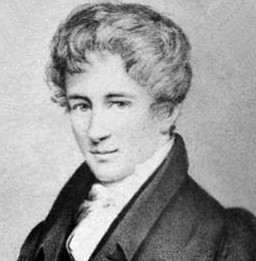
\includegraphics[scale=0.15]{Niels_Henrik_Abel} & 
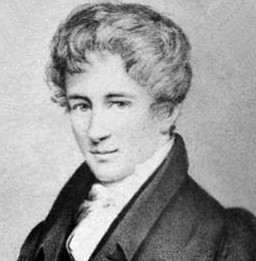
\includegraphics[scale=0.15,angle=-90,origin=c]{Niels_Henrik_Abel} & 
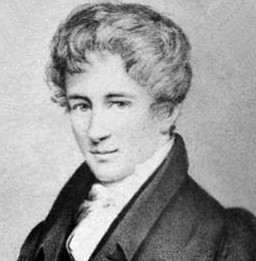
\includegraphics[scale=0.15,angle=180,origin=c]{Niels_Henrik_Abel} &
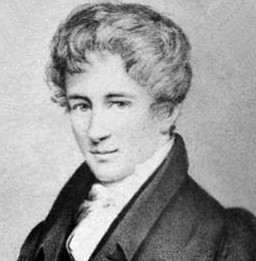
\includegraphics[scale=0.15,angle=90,origin=c]{Niels_Henrik_Abel} \\
$e$ & $r$ & $r^2$ & $r^3$ \\
&&& \\[-0.5pc]
\reflectbox{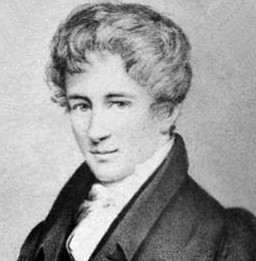
\includegraphics[scale=0.15]{Niels_Henrik_Abel}} & 
\reflectbox{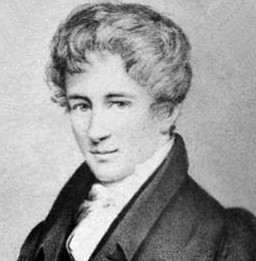
\includegraphics[scale=0.15,angle=-90,origin=c]{Niels_Henrik_Abel}} & 
\reflectbox{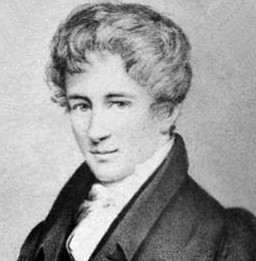
\includegraphics[scale=0.15,angle=180,origin=c]{Niels_Henrik_Abel}} &
\reflectbox{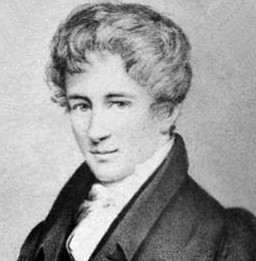
\includegraphics[scale=0.15,angle=90,origin=c]{Niels_Henrik_Abel}} \\
$s$ & $rs$ & $r^2s$ & $r^3s$ 
\end{tabular}
}

%\smallGap
\begin{que}
Why is the action of $D_4$ qualified as a \emph{right} action?
\end{que}
\end{frame}

% % %
\begin{frame}
\begin{exe}[cf. Problem 40]\label{exe:prob40}
\begin{enumerate}[(a)]
\item Complete the \vocab{multiplication table} for $D_4$.
\[
\begin{array}{c | c c c c c c c c}
 D_4  & e & r & r^2 & r^3 & s & rs & r^2s & r^3s \\
 \hline
 e & e & & & & & & & \\ 
 r & r & r^2 & r^3 & e & rs & r^2s & r^3s & s \\
 r^2 & & & & & & & & \\
 r^3 & & & & & & & & \\
 s & & & & & & & & \\
 rs & & & & & & & & \\
 r^2s & & & & & & & & \\
 r^3s & & & & & & & &
 \end{array}
\]
\item For each element in $D_4$, write down its inverse.
\item Prove $D_4$ is not abelian.
\end{enumerate}
\end{exe}
\end{frame}

% % % % %
\subsection[\subsecname]{Permutation groups}
% % %
\begin{frame}[c]{\subsecname}{}
Another special class of groups are the \vocab{permutation groups}.

\smallGap
\begin{dfn}
A \vocab{permutation} of a set $S$ is a bijection $\sigma:S\to S$.
\end{dfn}

\smallGap
\begin{exe}\label{exe:permutations}
\textbf{(Prove:)} Given a fixed set $S$ with finitely many elements, the set of permutations on $S$ forms a group under composition.
\end{exe}
\end{frame}

% % %
\begin{frame}[c]
\begin{dfn}
The group of permutations of the set $\{1,2,\dots,n\}$ is called the \vocab{symmetric group of order $n$}, and is denoted $S_n$.
\end{dfn}

\smallGap
\begin{exe}\label{exe:permAbelian}
For which values of $n$ is the permutation group $S_n$ abelian?
\end{exe}
\end{frame}

% % %
\begin{frame}
\begin{ex}\label{ex:permMatrices1}
One way to denote elements in $S_n$ is using matrices.  For example, the matrix
\[
\sigma=\begin{pmatrix}
	1 & 2 & 3 & 4 & 5 \\
	3 & 1 & 5 & 4 & 2
	\end{pmatrix}\in S_5
\]
represents the permutation
\begin{align*}
\sigma:\{1,2,3,4,5\} &\to \{1,2,3,4,5\} \\
	1 &\mapsto 3 \\
	2 &\mapsto 1 \\
	3 &\mapsto 5 \\
	4 &\mapsto 4 \\
	5 &\mapsto 2.
\end{align*}
\end{ex}
\end{frame}

% % %
\begin{frame}[c]
\textbf{Caution:} In this manner the elements of $S_n$ are not really matrices because their composition does not coincide with the usual matrix multiplication.

\smallGap
Rather, we have $n\times n$ \vocab{permutation matrices}, whose left multiplication permutes the rows of an $n\times n$ matrix, and whose right multiplication of the inverse (equivalently, transpose) permutes the columns.  
\end{frame}

% % %
\begin{frame}
\begin{ex}
We demonstrate the permutation $\sigma$ from Example \ref{ex:permMatrices1} on the rows of the an upper triangular matrix:
\[
\underbrace{\begin{pmatrix}
	0 & 1 & 0 & 0 & 0 \\
	0 & 0 & 0 & 0 & 1 \\
	1 & 0 & 0 & 0 & 0 \\
	0 & 0 & 0 & 1 & 0 \\
	0 & 0 & 1 & 0 & 0
	\end{pmatrix}}_{\sigma}
\begin{pmatrix}
	1 & * & 0 & 0 & 0 \\
	0 & 1 & 0 & 0 & 0 \\
	0 & 0 & 1 & 0 & 0 \\
	0 & 0 & 0 & 1 & 0 \\
	0 & 0 & 0 & 0 & 1
	\end{pmatrix} =
	\begin{pmatrix}
	0 & 1 & 0 & 0 & 0 \\
	0 & 0 & 0 & 0 & 1 \\
	1 & * & 0 & 0 & 0 \\
	0 & 0 & 0 & 1 & 0 \\
	0 & 0 & 1 & 0 & 0
	\end{pmatrix}
\]
and the columns:
\[
\begin{pmatrix}
	1 & * & 0 & 0 & 0 \\
	0 & 1 & 0 & 0 & 0 \\
	0 & 0 & 1 & 0 & 0 \\
	0 & 0 & 0 & 1 & 0 \\
	0 & 0 & 0 & 0 & 1
	\end{pmatrix}
\underbrace{\begin{pmatrix}
	0 & 0 & 1 & 0 & 0 \\
	1 & 0 & 0 & 0 & 0 \\
	0 & 0 & 0 & 0 & 1 \\
	0 & 0 & 0 & 1 & 0 \\
	0 & 1 & 0 & 0 & 0
	\end{pmatrix}}_{\sigma\1=\sigma\T} =
\begin{pmatrix}
* & 0 & 1 & 0 & 0 \\
1 & 0 & 0 & 0 & 0 \\
0 & 0 & 0 & 0 & 1 \\
0 & 0 & 0 & 1 & 0 \\
0 & 1 & 0 & 0 & 0
\end{pmatrix}	
\]
\end{ex}
\end{frame}

% % % % %
\subsection[\subsecname]{Monoids}\label{subsec:monoids}
% % %
\begin{frame}{\subsecname}
In Exercise \ref{exe:prob41} some of the set/operation pairs listed were not groups, but satisfied most of the required axioms.  In fact, there is a more general notion of such a pair.

\smallGap
\begin{dfn}
A \vocab{monoid} $M=(M,\star)$ is a set $M$, for which the following properties hold:
\begin{itemize}
\item $\star$ is a binary operation on $M$
\item $\star$ is associative
\item $M$ contains an identity element with respect to $\star$
\end{itemize}

\smallGap
A monoid is \vocab{commutative} means $a\star b=b\star a$ for all $g,h\in M$.
\end{dfn}
\end{frame}

% % %
\begin{frame}%[c]
Some authors refer to monoids as \vocab{semigroups}, and the difference is the presence of the identity element -- there is no convention on which term refers to which situation, so most authors specify or else use the terms \emph{monoid} and \emph{semigroup} interchangeably.

\smallGap
\begin{que}
All groups are monoids.  What is the missing axiom that makes a monoid, in general, not a group?
\end{que}

\smallGap
\begin{ex}
Given a directed graph $\Gamma$ with a global sink, the set $\mathscr M(\Gamma)$ of all stable sandpiles forms a monoid, known as the \vocab{sandpile monoid of $\Gamma$}.  (See Exercise \ref{exe:prob42}.)
\end{ex}
\end{frame}

% % %
\begin{frame}
\begin{ex}\label{ex:multGroup}
$\Q$ is a group under addition, but not multiplication -- the element $0$ has no inverse.  However, $\Q$ is a monoid under multiplication.  For this reason, when we refer to $\Q$ as a group, its implied operation is always addition.

\smallGap
On the other hand, $\Q^{\times}$ is a group under multiplication (hence, the name).  
\end{ex}

%\smallGap
\begin{que}
Is $\Q^{\times}$ a group under addition?
\end{que}

%\smallGap
\begin{exe}\label{exe:Zmonoid}
Prove the statements in Example \ref{ex:multGroup}:
\begin{enumerate}[(a)]
\item $\Q$ is a group under addition, but not multiplication.
\item $\Q$ is monoid under multiplication.
\item $\Q^{\times}$ is a group (implied operation is multiplication).
\end{enumerate}
\end{exe}
\end{frame}

% % %
\begin{frame}{}{}
\begin{ex}\label{ex:QRCmonoid}
Example \ref{ex:multGroup} also applies when we replace $\Q$ with $\R$ or $\C$.
\end{ex}

\smallGap
Recall, from Example \ref{ex:sets}, the use of $R$ to denote $\Z$, $\Q$, $\R$, and $\C$.  These groups have more in common than what is stated in Examples \ref{ex:multGroup} and \ref{ex:QRCmonoid}.  In particular, they all have a nice structure relating the additive and multiplicative operations via distribution; for $a,b,c\in R$, (where $R=\Z$, $\Q$, $\R$, or $\C$),
\[
a(b+c)=ab+ac.
\]
With this property, along with being an abelian group under addition, $R$ is called a \vocab{ring}.  Commutative Algebra revolves around the study of \vocab{commutative rings}, those whose multiplication is commutative.  

\smallGap
Unlike rings, monoids are \emph{less} structured than groups, not more, yet they still have many applications.  
\end{frame}

% % %
\begin{frame}
For example, the possible exponents in monomials in a polynomial ring can be indexed by vectors whose entries are integers.  These vectors form a monoid.

\smallGap
\begin{ex}\label{ex:semigroupRings}
Let $\R[x,y]$ denote the ring of polynomials in two variables with real coefficients and consider the three vectors $(5,2)$, $(0,1)$, and $(3,2)$ in $\Z^2$.  We form a monoid 
\[
M=\N\{(5,2),(0,1),(3,2)\}
\]
consisting all possible sums of $(5,2)$, $(0,1)$, and $(3,2)$ with coefficients in $\N$.  The corresponding semigroup ring is 
\[
R=\R[x^5y^2,y,x^3y^2]\subset \R[x,y],
\]
consisting of sums of monomials that are multiples of $x^5y^2$, $y$, and $x^3y^2$, with real coefficients.
\end{ex}
\end{frame}

% % % % %
\answerKey
% % %
\begin{frame}{\subsecname}
\exeSol[(cf. Problem 38)]{exe:functions}
\begin{itemize}
\item[(a)] \textbf{Well-defined;} assume $n\overset{\varphi_1}{\longmapsto} a$ and $n\overset{\varphi_1}{\longmapsto} b$, but $a\neq b$.  Then $\sqrt a\neq \sqrt b$.  But $\sqrt a=|n|$ and $\sqrt b=|n|$, a contradiction.  So $a=b$.

\smallGap
\textbf{Not injective;} $-1\neq 1$, but $\varphi_1(-1)=(-1)^2=1=1^2=\varphi_1(1)$.

\smallGap
\textbf{Not surjective;} $-1$ does not have a square root in $\Z$.

\smallGap
\item[(b)] \textbf{Well-defined;} assume $n\overset{\varphi_2}{\longmapsto} a$ and $n\overset{\varphi_2}{\longmapsto}b$, but $a\neq b$.  Then we have
\begin{align*}
a &\neq b \\
a(5n+1) &\neq b(5n+1) \\
2 & \neq 2,
\end{align*}
a contradiction.  So $a=b$.
\end{itemize}
\end{frame}

% % %
\begin{frame}
\begin{itemize}
\item[] \textbf{Injective;} suppose $\varphi_2(n)=\varphi_2(m)$.  Then we have
\begin{align*}
{\textstyle\frac{2}{5n+1}} &= \textstyle{\frac{2}{5m+1}} \\
2(5m+1) &= 2(5n+1) \\
5m+1 &= 5n+1 \\
5m &= 5n \\
m &= n.
\end{align*}

\smallGap
\textbf{Not surjective;} $0\in \Q$ but $0$ does not divide $2$.

\smallGap
\item[(c)] \textbf{Well-defined;} assume $(n,m)\overset{\varphi_3}{\longmapsto}a$ and $(n,m)\overset{\varphi_3}{\longmapsto}b$ but $a\neq b$.  Then we have 
\begin{align*}
a &\neq b \\
\log_n(a) &\neq \log_n(b) \\
m &\neq m,
\end{align*}
a contradiction.
\end{itemize}
\end{frame}

% % %
\begin{frame}
\begin{itemize}
\item[] \textbf{Not injective;} let $n_1=n_2=0$, $m_1=1$, $m_2=2$.  Then
\begin{align*}
(n_1,m_1) &\mapsto 0^1=0 \\
(n_2,m_2) &\mapsto 0^2=0
\end{align*}
but $(n_1,m_1)\neq (n_2,m_2)$.

\smallGap
\textbf{Surjective;} Choose $a\in\Z$.  Then $\varphi_3(a,1)=a^1=a$.  

\smallGap
\item[(d)] \textbf{Not a function;} if $\varphi_4(0)=0\notin\{\pm 1\}$.
\end{itemize}
\end{frame}

% % %
\begin{frame}
\exeSol[(cf. Problem 39)]{exe:binary}
\begin{itemize}
\item[(a)]\textbf{Binary;} writing $n\star m$, with $\star$ operating on $\N$, implies both $n$ and $m$ are natural numbers.  And, since $\N$ is well-defined (because it is a set -- cf. the definition!), the image of any pair $(n,m)$ is unique, namely, it is $n$.

\smallGap
\item[(b)]\label{sol:binary(b)} \textbf{Not binary;} as a counterexample, 1 and 2 are both natural numbers; $1\ominus 2=1-2=-1$ is not a natural number. 

\smallGap
\item[(c)] \textbf{Binary;} subtracting $n-m$ is the same as adding $n+(-m)$ and since the domain is $\Z$ we can write $\ominus(n,-m)=n+m$.  Addition is binary on $\Z$, hence so is subtraction.  

\smallGap
The \vocab{ambient set} of a binary operator matters!  When the context is not clear we may write $(\star, S)$ when referring to the binary operation $\star$ on $S$.  In this example we distinguish between $(\ominus, \N)$, subtraction on the natural numbers, and $(\ominus, \Z)$, subtraction on the integers.
\end{itemize}
\end{frame}

% % %
\begin{frame}
\begin{itemize}
\item[(d)] \textbf{Not binary;} Say $n=-1$ and $m=0$.  Then $2^{-1+0}=
\frac{1}{2}\notin \Z$.

%\textbf{Binary;} to prove, we shall express $(\odot,\mathbb Z)$ in terms of a handful of simpler operations:
	%\begin{itemize}\footnotesize
	%\item Since multiplication is binary on $\Z$, the map 
	%\begin{align*}
	%\varphi:\Z & \to \Z \\
	%	n & \mapsto n\times 2
	%\end{align*}
	%is well-defined. As a consequence, so is $\varphi\circ\varphi$.  Inductively, if we suppose for some $m\geq 2$, the composition
	%\[
	%\varphi^m:=\underbrace{\varphi\circ\dots\circ\varphi}_{\text{$m$ times}}
	%\]
	%is well-defined, then $\image(\varphi^m)\subset\Z$ and so $\varphi^{m+1}:=\varphi^m\circ\varphi$ must also be well-defined.
	%
	%\smallGap
	%\item Using the fact that multiplication is binary on $\Q$ and $\Z\subset \Q$, define
	%\begin{align*}
	%\psi: \Z & \to \Q \\
	%	n & \mapsto {\textstyle\frac{1}{2}}n
	%\end{align*}
	%\end{itemize}
%\end{itemize}
%\end{frame}
%
% % %
%\begin{frame}
%\begin{itemize}
%\item[]\begin{itemize}\footnotesize
%	\item[] and then use the same arguments to show $\psi$ and all of its ``powers" $\psi^m$ are well-defined.
%	\item Finally, define
%	\vspace{-0.25pc}
%	\begin{align*}
%	\rho : \Z & \to \Z^{\Q} \\
%		n & \mapsto \begin{cases}
%			\varphi^n & n> 0 \\
%			1 & n=0 \\
%			\psi^{-n} & n<0,
%			\end{cases}
%	\end{align*} 
%	well-defined since its image can be identified with the integers (we say the image is in \vocab{bijection} or \vocab{one-to-one correspondence} with $\mathbb Z$), meaning we can ``match" each element in $\image(\rho)$ with a unique integer.
%	
%	\smallGap
%	The point is that $\rho$ will correspond to raising $2$ to various integer powers.
%	\end{itemize}
%
%\smallGap	
%We now can write $n\odot m=\rho(n+m)(1)$, which is the function $\rho(n+m):\Z\to \Q$, evaluated at the element $1$.  The image of $\odot$ is a union of the images of $\rho(n+m)$, for all possible pairs $n+m\in \Z$, and these images are all contained in $\Z$.  It follows that $\image{(\odot)}$ is a subset of $\Z$ and hence it follows that $\odot$ is well-defined. 
%\qed	
%\end{itemize}
%\end{frame}
%
% % %
%\begin{frame}
%\begin{itemize}
\item[(e)] \textbf{Not binary;} the pair $(0,0)\in\Q\times \Q$, but $\varphi_3(0,0)=0^0$ is an indeterminant form, so is not in $\Q$.   

\smallGap
\item[(f)] \textbf{Binary;} if $f,g\in S^S$ then for any $s\in S$, $f(s)\in S$ and so $g\left(f(s)\right)\in S$.  

\smallGap
\item[(g)] \textbf{Not binary;} $S=\N$, $T=\Q$ provides a counterexample: The map
\begin{align*}
\varphi:\N & \to \Q \\
	n & \mapsto {\textstyle\frac{n}{2}}
\end{align*}
is well-defined because division is well-defined on $\Q^{\times}$ and $\N\subset \Q^{\times}\subset \Q$.  But $\varphi$ cannot be composed with itself: If $n=1$ then
\begin{align*}
f\circ f(1) & = f\left(f(1)\right) \\
	& = f\left({\textstyle\frac{1}{2}}\right) 
\end{align*}
but $\frac{1}{2}$ is not in the domain, $\N$.
\end{itemize}
\end{frame}

% % %
\begin{frame}
\exeSol[(cf. Problem 41)]{exe:prob41}
\begin{itemize}
\item[(a)] \textbf{Abelian group;} the operation $\cdot$ is binary because the product of two positive rational numbers is positive and rational.  Associativity holds from ``order of operations" rules for multiplication.  The identity element is $1$ since for any $q\in\Q^+$, $1\cdot q=q\cdot 1=q$.  And, an element $q\in\Q^+$ has inverse $\frac{1}{q}$, since $q\cdot\frac{1}{q}=\frac{1}{q}\cdot q=1$.

\smallGap
Finally, $(\Q^+,\cdot)$ is abelian because multiplication is a commutative operation in $\R$, and $\Q^+\subset \R$.  

\smallGap
\item[(b)] \textbf{Not a group;} associativity fails, since
\[
(1-1)-1=-1\; \neq 1=1-(1-1).
\]

\smallGap
\item[(c)] \textbf{Not a group;} associativity fails since 
\[
(1\div 2)\div 3=\frac{\frac{1}{2}}{3}=\frac{1}{2\cdot 3}=\frac{1}{6},
\]
while 
\[
1\div (2\div 3)=\frac{1}{\frac{2}{3}}=\frac{1\cdot 3}{2}=\frac{3}{2}.
\]
\end{itemize}
\end{frame}

% % %
\begin{frame}
\begin{itemize}
\item[(d)] \textbf{Abelian group;} any remainder upon division by $12$ is between $0$ and $11$, inclusive, so $\oplus_{12}$ is binary.  Associativity holds because modular arithmetic is associative:
\begin{align*}
(a\oplus_{12}b)\oplus_{12}c &= (a+b\mod{12})+c\mod{12} \\
	&= a+b+c\mod{12} \\
	&= a\mod{12}+(b+c\mod{12}) \\
	&= a\oplus_{12}(b\oplus_{12}c)
\end{align*}
The identity element is 0, and in $\Z$.  The inverse elements are given as follows:

\vspace{-1pc}
\begin{tabular}{p{0.25\textwidth}p{0.25\textwidth}p{0.25\textwidth}}
{\begin{align*}
-0 &= 0 \\
-1 &= 11 \\
-2 &= 10 \\
-3 &= 9 
\end{align*}
}
&
{\begin{align*}
-4 &= 8 \\
-5 &= 7 \\
-6 &= 6 \\
-7 &= 5 
\end{align*}
}
&
{\begin{align*}
-8 &= 4 \\
-9 &= 3 \\
-10 &= 2 \\
-11 &= 1 
\end{align*}
}
\end{tabular}

\smallGap Finally, $\Z_{12}$ is abelian because addition is commutative in $\Z$.

\smallGap
\textbf{Note:} Understanding $\Z_{12}$ and similar groups will be very important to the sandpile research projects.
\end{itemize}
\end{frame}

% % %
\begin{frame}
\begin{itemize}
\item[(e)] \textbf{Non-abelian group;} suppose $M_1,M_2\in\GL(2,\R)$.  For multiplication to be binary in $GL(2,\R)$ we need to make sure $M_1\cdot M_2$ is invertible.  Since $M_1,M_2$ each have inverses by hypothesis,
\[
(M_1\cdot M_2)\1=M_2\1\cdot M_1\1.
\]
For associativity, take $\Big(\begin{smallmatrix} a_1 & a_2 \\[2.5pt] a_3 & a_4 \end{smallmatrix}\Big)$, $\left(\begin{smallmatrix} b_1 & b_2 \\ b_3 & b_4 \end{smallmatrix}\right)$, and $\Big(\begin{smallmatrix} c_1 & c_2 \\[2.5pt] c_3 & c_4 \end{smallmatrix}\Big)$ in $\GL(2,\R)$.  Then:
\begin{align*}
	&\left(\begin{pmatrix}
	a_1 & a_2 \\
	a_3 & a_4 
	\end{pmatrix}\cdot
	\begin{pmatrix}
	b_1 & b_2 \\
	b_3 & b_4 
	\end{pmatrix}
	\right)\cdot
	\begin{pmatrix}
	c_1 & c_2 \\
	c_3 & c_4
	\end{pmatrix} \\
=& \begin{pmatrix}
	a_1b_1 + a_2b_3 & a_1b_2 + a_2b_4 \\
	a_3b_1 + a_4b_3 & a_3b_2 + a_4b_4
	\end{pmatrix}\cdot 
	\begin{pmatrix}
	c_1 & c_2 \\
	c_3 & c_4
	\end{pmatrix} \\
=& \begin{pmatrix}
a_1b_1c_1 + a_2b_3c_1 + a_1b_2c_3 + a_2b_4c_3 & 
	a_1b_1c_2 + a_2b_3c_2 +a_1b_2c_4 + a_2b_4c_4 \\
a_3b_1c_1 + a_4b_3c_1 + a_3b_2c_3 + a_4b_4c_3 & 
	a_3b_1c_2 + a_4b_3c_2 +a_3b_2c_4 + a_4b_4c_4	
\end{pmatrix} \\
=& \begin{pmatrix}
a_1(b_1c_1+b_2c_3) + a_2(b_3c_1+b_4c_3) &
	a_1(b_2c_2+b_2c_4) + a_2(b_3c_2+b_4c_4) \\
a_3(b_1c_1+b_2c_3) + a_4(b_3c_1+b_4c_3) &
	a_3(b_2c_2+b_2c_4) + a_4(b_3c_2+b_4c_4) 
\end{pmatrix} \\
=& \begin{pmatrix}
	a_1 & a_2 \\
	a_3 & a_4
	\end{pmatrix}\cdot
	\begin{pmatrix}
	b_1c_1+b_2c_3 & b_2c_2+b_2c_4 \\
	b_3c_1+b_4c_3 & b_3c_2+b_4c_4
	\end{pmatrix} \\
=& \begin{pmatrix}
	a_1 & a_2 \\
	a_3 & a_4
	\end{pmatrix}
	\cdot
	\left(\begin{pmatrix}
		b_1 & b_2 \\
		b_3 & b_4
		\end{pmatrix}
		\cdot
		\begin{pmatrix}
		c_1 & c_2 \\
		c_3 & c_4
		\end{pmatrix}
		\right)
\end{align*}
\end{itemize}
\end{frame}

% % %
\begin{frame}
The identity element is the identity matrix.  Say $\left(\begin{smallmatrix}a & b \\ c & d \end{smallmatrix}\right)\in\GL(2,\R)$.  Then
\[
\begin{pmatrix}
a & b \\
c & d
\end{pmatrix}
\cdot\begin{pmatrix}
1 & 0 \\
0 & 1
\end{pmatrix}=
\begin{pmatrix}
a & b \\
c & d
\end{pmatrix}=
\begin{pmatrix}
1 & 0 \\
0 & 1
\end{pmatrix}
\cdot
\begin{pmatrix}
a & b \\
c & d
\end{pmatrix}
\]
$\GL(2,\R)$ has inverses, by definition.  

\smallGap
$\GL(2,\R)$ is not abelian.  We exhibit a counterexample using matrices whose respective determinants are $1$ and $-1$ (verifying they are invertible).
\begin{align*}
\underbrace{\begin{pmatrix}
	1 & 0 \\
	1 & 1
	\end{pmatrix}}_{\det{}=1}\cdot
\underbrace{\begin{pmatrix}
	0 & 1 \\
	1 & 1 
\end{pmatrix}}_{\det{}=-1} &=
\begin{pmatrix}
0 & 1 \\
1 & 2
\end{pmatrix} \\
\begin{pmatrix}
	0 & 1 \\
	1 & 1
	\end{pmatrix}\cdot
\begin{pmatrix}
	1 & 0 \\
	1 & 1 
\end{pmatrix} &=
\begin{pmatrix}
1 & 1 \\
2 & 1
\end{pmatrix}
\end{align*}
\end{frame}

% % %
\begin{frame}[fragile]
\exeSol[(cf. Problem 42)]{exe:prob42}
\begin{itemize}
\item[(a)] We use Sage to draw $\Gamma$ and list the elements of $\mathscr S(\Gamma)$, which is denoted \verb|SGam| in the code.

%\vspace{-0.2pc}
%\begin{center}
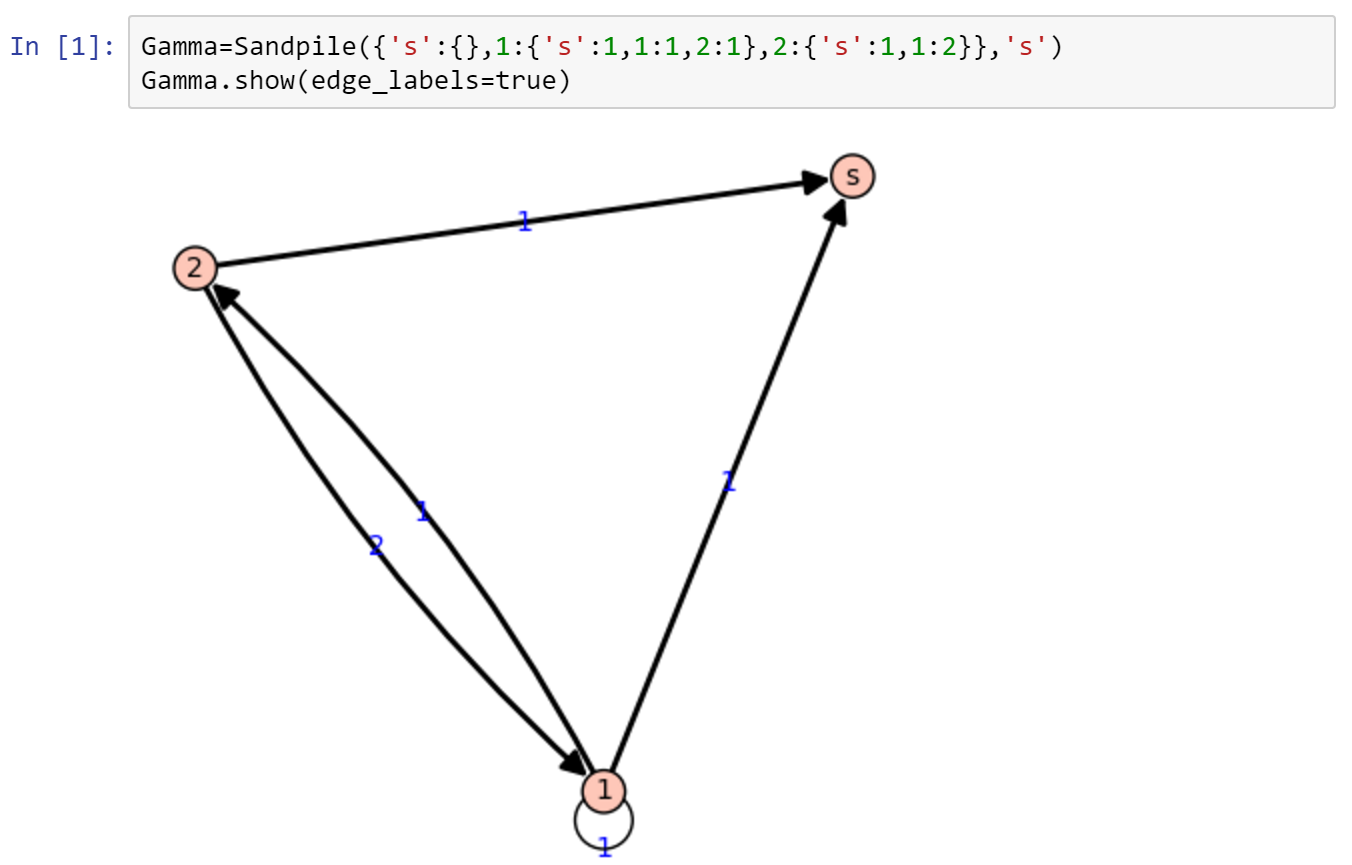
\includegraphics[scale=0.46]{sageFig1-1}
%\end{center}
\end{itemize}
\end{frame}

% % %
\begin{frame}[fragile,c]
\begin{itemize}
\item[] %\begin{center}
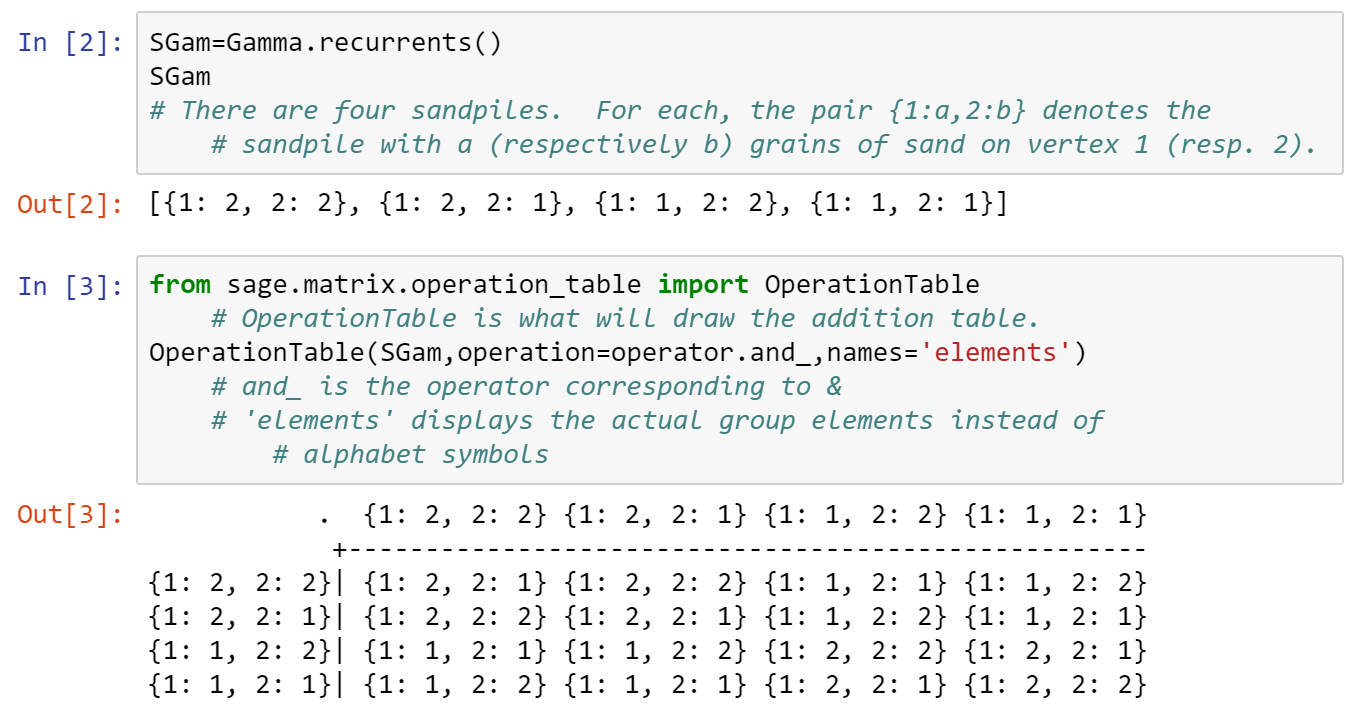
\includegraphics[scale=0.46]{sageFig1-1pt2}
%\end{center}

In the third cell (\verb|Out[3]|) we display the addition table for $\mathscr S(\Gamma)$, showing stable addition is a binary operation.  From the table, the identity element is given by the sandpile 
\[
e:=\{\verb|1:2,2:1|\}=(2,1).
\]
\end{itemize}
\end{frame}

% % %
\begin{frame}
\begin{itemize}
\item[] Associativity also follows from the table and from Problem 27.  The inverses are listed as follows:
\begin{align*}
(2,2)\1 &= (2,2) \\
(2,1)\1 &= (2,1) \\
(1,2)\1 &= (1,1) \\
(1,1)\1 &= (1,2)
\end{align*}
\qed

\smallGap
\item[(b)] To show $\mathscr M(\Gamma)$ is not a group we exhibit an element without an inverse.  The sandpile $c=(1,0)$ is stable, but has no inverse under stable addition.
\qed
\end{itemize}
\end{frame}

% % %
\begin{frame}
\exeSol[(cf. Problem 40)]{exe:prob40}
\begin{itemize}%[(a)]
\item[(a)] $\displaystyle
\begin{array}[t]{c | c c c c c c c c}
 D_4  & e & r & r^2 & r^3 & s & rs & r^2s & r^3s \\
 \hline
 e & e & \vect{{r}} & \vect{{r^2}} & \vect{{r^3}} & \vect{{s}} & \vect{{rs}} & \vect{{r^2s}} & \vect{{r^3s}} \\ 
 r & r & r^2 & r^3 & e & rs & r^2s & r^3s & s \\
 r^2 & \vect{{r^2}} & \vect{{r^3}} & \vect{{e}} & \vect{{r}} & \vect{{r^2s}} & \vect{{r^3s}} & \vect{{s}} & \vect{{rs}} \\
 r^3 & \vect{{r^3}} & \vect{{e}} & \vect{{r}} & \vect{{r^2}} & \vect{{r^3s}} & \vect{{s}} & \vect{{rs}} & \vect{{r^2s}} \\
 s & \vect{{s}} & \vect{{r^3s}} & \vect{{r^2s}} & \vect{{rs}} & \vect{{e}} & \vect{{r^3}} & \vect{{r^2}} & \vect{{r}} \\
 rs & \vect{{rs}} & \vect{{s}} & \vect{{r^3s}} & \vect{{r^2s}} & \vect{{r}}  & \vect{{e}} & \vect{{r^3}} & \vect{{r^2}} \\
 r^2s & \vect{{r^2s}} & \vect{{rs}} & \vect{{s}} & \vect{{r^3s}} & \vect{{r^2}} & \vect{{r}} & \vect{{e}} & \vect{{r^3}} \\
 r^3s & \vect{{r^3s}} & \vect{{r^2s}} & \vect{{rs}} & \vect{{s}} & \vect{{r^3}} & \vect{{r^2}} & \vect{{r}} & \vect{{e}}
 \end{array}
$

\smallGap
\item[(b)]
\begin{tabular}[t]{p{0.2\textwidth}p{0.2\textwidth}}
\vspace{-1.1pc}
{\begin{align*}
e\1 &= e \\
r\1 &= r^3 \\
(r^2)\1 &= r^2 \\
(r^3)\1 &= r
\end{align*}
} 
& \vspace{-1.1pc}
{\begin{align*}
s\1 &= s \\
(rs)\1 &= rs \\
(r^2s)\1 &= r^2s \\
(r^3s)\1 &= r^3s
\end{align*}
}
\end{tabular}

\vspace{-1pc}
\item[(c)] From the multiplication table, $rs\neq sr=r^3s$.
\end{itemize}
\end{frame}

% % % 
\begin{frame}
\exeSol[(cf. notes)]{exe:permutations}
Permutations are bijective, so composing them results in a bijection.  Therefore composition is a binary operation on the set of permutations of $S$.  To see associativity, take $x\in S$ and $\sigma$, $\tau$, and $\nu$ in $S_n$.  Then apply the permutations to $x$:
\begin{align*}
(\sigma\circ\tau)\circ \nu(x) &= (\sigma\circ\tau)\left(\nu(x)\right) \\
 &= \sigma\left(\tau\left(\nu(x)\right)\right); \\
\sigma\circ(\tau\circ\nu)(x) &= \sigma\left(\tau\circ\nu(x)\right) \\
 &= \sigma\left(\tau\left(\nu(x)\right)\right).  
\end{align*}
The identity element is the permutation that does nothing, so composing with any other permutation $\sigma$ is the same as just applying $\sigma$.  Finally, all permutations are bijections and so have inverses.
\qed
\end{frame}

% % %
\begin{frame}
\exeSol{exe:permAbelian}
$S_1$ consists of one element so is vacuously abelian; $S_2$ contains two elements, one of which is the identity, which commutes with the other.

\smallGap
In $S_3$ consider the permutations
\begin{tabular}{p{0.4\textwidth}p{0.4\textwidth}}
\vspace{-0.75pc}
{\begin{align*}
\sigma: \{a,b,c\} &\to \{a,b,c\} \\
	a &\mapsto c \\
	b &\mapsto b \\
	c &\mapsto a
\end{align*}
} & \vspace{-0.75pc}
{\begin{align*}
\tau: \{a,b,c\} &\to \{a,b,c\} \\
	a &\mapsto b\\
	b &\mapsto c\\
	c &\mapsto a
\end{align*}
}
\end{tabular}

\vspace{-0.75pc}
Then, composing from left to right:
\begin{tabular}{p{0.4\textwidth}p{0.4\textwidth}}
\vspace{-0.75pc}
{\begin{align*}
\sigma\tau: \{a,b,c\} &\to \{a,b,c\} \\
	a &\mapsto a \\
	b &\mapsto c \\
	c &\mapsto b
\end{align*}
} & \vspace{-0.75pc}
{\begin{align*}
\tau\sigma: \{a,b,c\} &\to \{a,b,c\} \\
	a &\mapsto b \\
	b &\mapsto a \\
	c &\mapsto c
\end{align*}
}
\end{tabular}
\end{frame}

% % %
\begin{frame}
To generalize to $n\geq 4$, take 
\begin{align*}
\sigma: \{a,b,c,\dots, \text{$n$th element}\} &\to \{a,b,c, \dots, \text{$n$th element}\} \\
	a &\mapsto c \\
	b &\mapsto b \\
	c &\mapsto a \\
	\text{each other element} &\mapsto \text{itself}
\end{align*}
and 
\begin{align*}
\tau: \{a,b,c,\dots,\text{$n$th element}\} &\to \{a,b,c,\dots,\text{$n$th element}\} \\
	a &\mapsto b \\
	b &\mapsto c \\
	c &\mapsto a \\
	\text{each other element} &\mapsto \text{itself}
\end{align*}

\smallGap
To summarize, $S_1$ and $S_2$ are abelian.  $S_n$ for $n\geq 4$ is not abelian.
\end{frame}

% % %
\begin{frame}
\exeSol{exe:Zmonoid}
\begin{itemize}
\item[(a)] We verify the group axioms for $\Q$:
\begin{itemize}\footnotesize
	\item Addition is binary on $\Q$; $\frac{n_1}{m_1}+\frac{n_2}{m_2}=\frac{n_1m_2+n_2m_1}{m_1m_2}\in \Q$ (with $m_1,m_2\neq 0$).
	\item We can also directly show addition is associative:
	\begin{align*}\textstyle
	\left(\frac{n_1}{m_1}+\frac{n_2}{m_2}\right)+\frac{n_3}{m_3} &= \textstyle \left(\frac{n_1m_2+n_2m_1}{m_1m_2}\right)+\frac{n_3}{m_3} \\
		&= \textstyle \frac{n_1m_2m_3+n_2m_1m_3+m_1m_2n_3}{m_1m_2m_3}; \\
	\textstyle \frac{n_1}{m_1}+\left(\frac{n_2}{m_2}+\frac{n_3}{m_3}\right) &= \textstyle \frac{n_1}{m_1}+\left(\frac{n_2m_3+n_3m_2}{m_2m_3}\right) \\
		&= \textstyle \frac{n_1m_2m_3+n_2m_1m_3+m_1m_2n_3}{m_1m_2m_3}
	\end{align*}
	\item The identity element is $0$, since for any $q\in \Q$, $0+q=q+0=q$.
	\item For any $q\in \Q$, its inverse is $-q$, because $q+(-q)=0$.
	
	\smallGap
	For multiplication this axiom fails, since $0$ has no inverse.
	\end{itemize}
\end{itemize}
\end{frame}

% % %
\begin{frame}
\begin{itemize}\footnotesize
\item[(b)] We verify the monoid axioms:
	\begin{itemize}\footnotesize
	\item Multiplication is binary, since $\frac{n_1}{m_1}\cdot\frac{n_2}{m_2}=\frac{n_1n_2}{m_1m_2}\in \Q$.
	\item Multiplication is associative, since 
	\[\textstyle
	\left(\frac{n_1}{m_1}\cdot \frac{n_2}{m_2}\right)\cdot \frac{n_3}{m_3}=\left(\frac{n_1n_2}{m_1m_2}\right)\cdot \frac{n_3}{m_3} = \frac{n_1n_2n_3}{m_1m_2m_3} = \frac{n_1}{m_1}\cdot \left(\frac{n_2n_3}{m_2m_3}\right) =
	\frac{n_1}{m_1}\cdot \left(\frac{n_2}{m_2}\cdot \frac{n_3}{m_3}\right).
	\]
	\item The multiplicative inverse is $1$, since given $q\in \Q$, $1\cdot q=q=q\cdot 1$.
	\end{itemize}	

\smallGap	
\item[(c)] The first three group axioms hold as shown above, since $\Q^{\times}\subset\Q$ and no product of non-zero elements results in $0$.  The only element in $\Q$ without an inverse was $0$, so all elements in $\Q=\Q\setminus\{0\}$ have inverses. 	
\end{itemize}
\end{frame}

% % % % % % % % % % % % % % % % % % % %
\end{document}